\documentclass[aip, amsmath, amssymb, preprint,floatfix]{revtex4-2}
\usepackage[utf8]{inputenc}
\usepackage{graphicx} % Required for including pictures

\usepackage[hidelinks]{hyperref}
\usepackage{xcolor}
\bibliographystyle{apsrev4-2}
\include{shortcuts}

\begin{document}
\title{Design Document\\APC 524}
\date{2021}

\author{Dingyun Liu, Bingjia Yang, Kehan Cai, and Tal Rubin}
\maketitle

\section{Introduciton}

Fluids are ubiquitous in physical systems of all sizes; astronomical-scale Magnetohydrodynamics, planetary weather models, rivers and pipe-flows, to the smallest blood-vessels. Fluids can describe liquids, gases and plasmas, and appear in the limit of short mean-free-path of a \textit{N}-body problem.

\section{Mathematical Model}

The mathematical description of fluids boils down to conservation laws. 

Conservation of mass, or particle number density is called the continuity equation, and is written in Eulerian form as,
\begin{gather}
	\pdv{n}{t} + \nabla \cdot (n \bv) = 0,
\end{gather}
with $n$ being the number density, $t$, the time, and $\bv$ the velocity vector.

The momentum evolution equation is,
\begin{gather}
    \pdv{\bP}{t} + \nabla \cdot\left(\bv \bP + p \bI + \pi\right) =  \bF,~\label{eq:momentum}
\end{gather}
with $\bP = m n \bv$ being the linear momentum vector, with $m$ denoting the mass of a fluid particle, $\bv \bP$ is a dyadic tensor, obtained by a tensor product of the velocity and momentum, $p$ is the scalar pressure, $\bI$ is the unit tensor, $\pi$ is the viscous stress tensor, and $\bF$ is the body force acting on a fluid element.

Possible body forces are Lorentz force for a fluid plasma, friction force for a multi-fluid system, gravity in the presence of a gravitational field. Other body forces can be fictitious such as centrifugal and Coriolis forces. The viscous stress introduces momentum diffusion.

In the case of $\bF=0$, the momentum equation becomes a conservation law:
\begin{gather}
    \pdv{\bP}{t} + \nabla \cdot\left(\bv \bP + p \bI + \pi\right) =  0.~\label{eq:momentum_conservation}
\end{gather}

In some fluid models (e.g. Navier–Stokes), these equations are sufficient to close the system of equations. In other models, an energy equation is added:
\begin{gather}
    \pdv{E}{t} + \nabla \cdot\left(\bv (E + p)+\bq\right) =  \bv\cdot\bF + Q,~\label{eq:energy}
\end{gather}
with $E$ being the internal energy of a fluid element, $\bq$ begin the heat diffusion, $\bv\cdot\bF$ is the work done on the fluid element by external forces, and $Q$ being energy source terms such as external heating.

Again, in the case of $\bv\cdot\bF = 0$ and $Q=0$, this is a conservation equation. 
\begin{gather}
    \pdv{E}{t} + \nabla \cdot\left(\bv (E + p)+\bq\right) =  0.~\label{eq:energy_conservation}
\end{gather}

\subsection{Finite volume and discontinuous Galerkin methods}

A popular numerical discretization of this equation set is the finite volume method. Assume the solution domain is divided into several non-overlapping ``control volumes", denoted by $C$. Integrating the equations over a cell yields,
\begin{gather}
	\int_C\pdv{n}{t}dV + \int_C \nabla \cdot (n \bv)dV = 0,
\end{gather}
with $dV$ being a volume element of the right dimensionality. Using $\overline X = \int_C X dV$, and $\hat n$ as the unit vector normal to the surface $\partial C$ of the volume $C$, the equations for the average density, momentum and energy in a volume become:
\begin{gather}
	\pdv{\overline n}{t} + \int_{\partial C} \hat n \cdot (n \bv)dS = 0,\\
    	\pdv{\overline \bP}{t} + \int_{\partial C} \hat n  \cdot\left(\bv \bP + p \bI + \pi\right)dS = \overline \bF,\\
    	\pdv{\overline E}{t} +  \int_{\partial C} \hat n \cdot \left(\bv (E + p)+\bq\right)dS =  \overline{\bv\cdot\bF}+ \overline Q,
\end{gather}
with $dS$ being a surface element of the right dimensionality.



























\section{Proposed work}

We propose to build a code capable of handling different fluid models, and different solvers.

The code would be split into three computational steps: 
\noindent
\begin{enumerate}
\item Pre-processor: \newline
Meshing, Initial conditions.
\item Solver: \newline
Time-stepping, Boundary conditions.
\item Post-processor: \newline
Visualization.
\end{enumerate}

A driver code would navigate between the code steps. The user would define a domain and the mesh parameters. The domain dimensionality would inform the fluid model selection (possibly by reducing the number of equations from 3D to the appropriate dimentionality).

It is likely we would attempt to use an external library for the mesher - as this is a complex task on its own. 


The user would define boundary conditions, and the fluid would be initilized with a quiesent initial conditions.

We would want to have a choice between ``regular" time-stepping algorithms such as Runge-Kutta or Adams-Moulton, and symplectic algorithms such as leap-frog, or a splitting method.

The user would also determine the time-limit for the integration and the frequency of data output. The solver would advanve the fluid in time using the selected time-stepping algorithm, and save the information.

The post-processor would visualize the resulting information. The post processor would be written in python.


We plan on using GitHub using a centralized workflow, in which the master branch is updated via pull requests. Current repository is \href{git@github.com:Tal-Rubin/APC524.git}{git@github.com:Tal-Rubin/APC524.git}.



\section{UML Diagram}
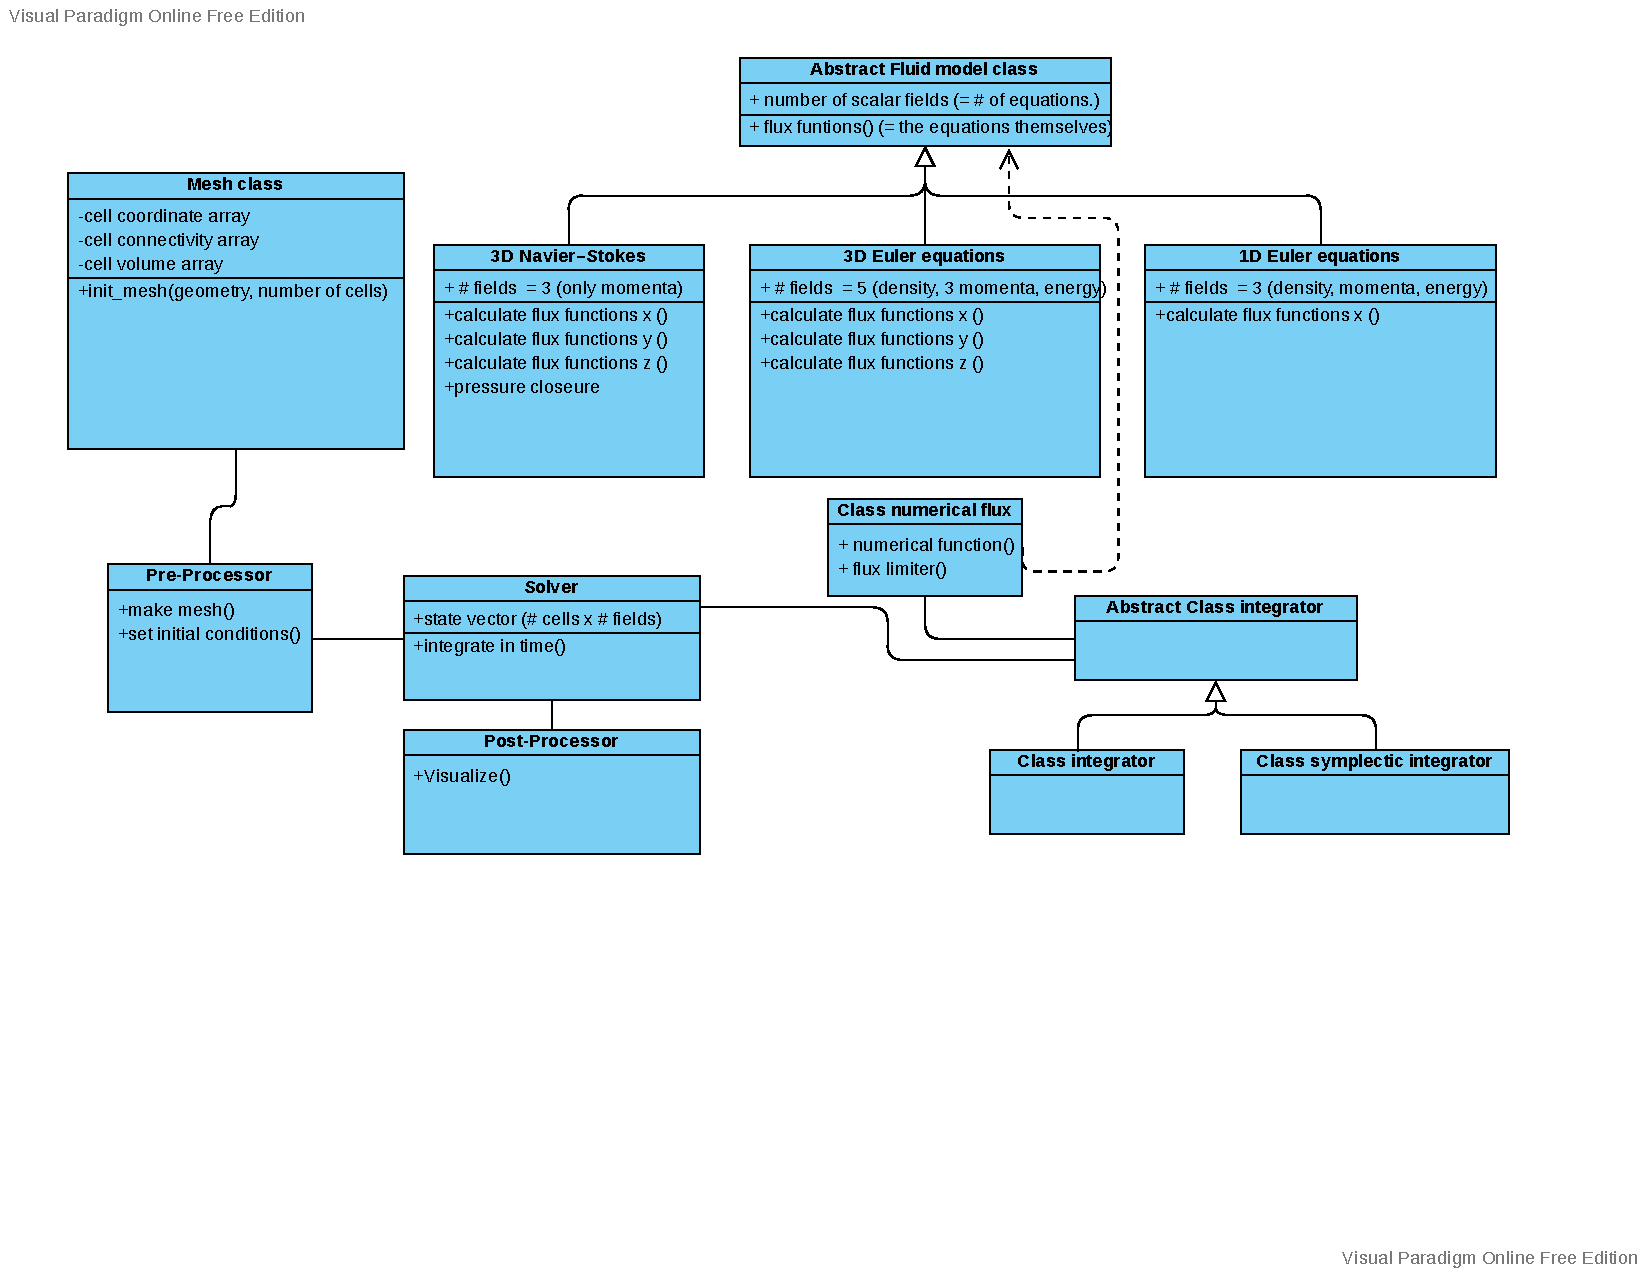
\includegraphics[width = \linewidth]{APC524UML.pdf}

\section{Milestones}

We have approximately one month to finish the alpha version, and about 2 weeks later the project is due.

The table below lists the major dates and milestones for the project.

\begin{tabular}{c|c|c}
    Week & Date & Task \\
    \hline
    1 & 31 Oct & Revise design document \\
    2 & 07 Nov & Git + CI setup \\
    3 & 14 Nov & Implement Riemann solver code \\
    4 & 22-23 Nov & Check-in with AIs \\
    5 & 30 Nov & Alpha version due \\
    6 & 7 Dec & Testing and code modifications \\
    7 & 14 Dec & Final version due \\
\end{tabular}







\end{document}